\begin{frame}{Tætslåede vegetationsstriber}

\small

\begin{columns}[T]

\begin{column}{0.58\textwidth}

\textbf{Regler for tætslåede vegetationsstriber:}

\begin{itemize}[]
\item Holdes kort ved hyppig slåning
\item Må ikke kunne indbyde til redeskjul
\item Min. 2 m brede
\item Max. 6 m brede
\item Min. 20 m mellem striberne
\end{itemize}

\vspace{0.4em}

\textbf{Gavner arter:}

\footnotesize
Vibe, sanglærke, markpiber, finke, agerhøne, gul vipstjert, 
rødrygget tornskade, gulspurv, vilde bier, humlebier, dagsommerfugle, 
svirrefluer, rovbiller, græshopper, markmus, pindsvin, musvåge, tårnfalk

\end{column}

\begin{column}{0.40\textwidth}
\centering
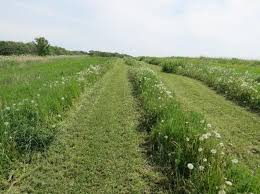
\includegraphics[width=\textwidth]{Billeder/Vildtforvaltning/biotopplantiltag/slået_vegetationsstribe.jpeg}
\end{column}

\end{columns}

\end{frame}